\chapter{Methodology}
\TODO{explain that we're using cartesian coords for everything.  See how Matt Jones justified this.}
\TODO{introduce the equation set and Hilary's discretisation}
\TODO{say something about how OpenFOAM always operates in 3D}

\section{Grid construction}
\label{sec:method:grid}

Two dimensional, regular cartesian grids were created using the OpenFOAM utility, \shellcmd{blockMesh}.  A custom utility was used to modify these orthogonal grids by adjusting the height of points to create terrain following grids.

At the time of writing, OpenFOAM does not directly support cut cell grids\footnote{An enhancement request was filed in 2013 to add support for cartesian cut cells to OpenFOAM, see \url{http://www.openfoam.org/mantisbt/view.php?id=1083}}.  Instead, the \shellcmd{snappyHexMesh} OpenFOAM utility was used to create a grid that approximates the cut cell method.  First, a custom utility was used to move points beneath the surface up to the surface creating small cells near mountain peaks.  Second, a description of the surface was taken from any of the terrain following grids and \shellcmd{snappyHexMesh} was used to intersect the surface with the grid.  The tool removes cells whose centres are below the surface.  An example of the resulting grid is shown in figure~\ref{fig:method:cut-cell}.

The grid is not strictly a cut cell mesh because, when \shellcmd{snappyHexMesh} moves points along the surface according to its heuristics, some points are moved horizontally.  It has not been possible to correct this issue for this project.  This grid is referred to as the `SnapCol' grid throughout this project.

\begin{figure}
	\centerfloat
	\includegraphics[height=2.8in,angle=270]{mesh-snapCol-schaerExp-resting.eps}
	\caption{A `SnapCol' grid created by intersecting the terrain surface with a regular grid as described in section~\ref{sec:method:grid}.  Note that, unlike a true cut cell grid, some small cells have faces at $z = \SI{500}{\meter}$ that are not entirely horizontal.}
	\label{fig:method:cut-cell}
\end{figure}

\section{Discretisation of Euler equations}
\label{sec:method:discretisation}
The fully-compressible Euler equations used in the resting atmosphere test (section~\ref{sec:resting}) and gravity waves test (section~\ref{sec:gw}) are specified as
\begin{align}
& \text{Momentum} & \frac{\partial \rho \vect{u}}{\partial t} + \del \cdot \rho \vect{u} \vect{u} &= \rho \vect{g} - c_p \rho \theta \del \exner \\
%
& \text{Continuity} & \frac{\partial \rho}{\partial t} + \del \cdot \rho \vect{u} &= 0 \\
%
& \text{Potential temperature (flux form)} & \frac{\partial \rho \theta}{\partial t} + \del \cdot \rho \vect{u} \theta &= 0 \\
%
& \text{Potential temperature (advective form)} & \frac{\partial \theta}{\partial t} + \vect{u} \cdot \del \theta &= 0 \\
%
& \text{Equation of state} & \exner^{(1 - \kappa / \kappa)} &= \frac{R \rho \theta}{p_0}
\end{align}
where $\rho$ is the density, $\vect{u}$ is the velocity field, $\vect{g}$ is gravitational acceleration, $c_p$ is the heat capacity of dry air at constant pressure, $\theta$ is the potential temperature, $\exner = \left( p / p_0 \right)^\kappa$ is the Exner function of pressure, $p$ is the pressure, $p_0$ is a reference pressure, $\kappa = R/c_p$, and $R$ is the specific gas constant of dry air.

Here, we outline the placement of prognostic variables, pressure gradient discretisation, and the advection scheme.  Further details of the discretisation are given by \textcite{weller-shahrokhi2014}.

\begin{figure}
	\captionsetup[subfigure]{position=b}
	\centering
	\subcaptionbox{Vertical cross section of geometry}[0.48\textwidth]{\documentclass[tikz]{standalone}
\usepackage{bm}
\newcommand{\vect}{\bm}
\newcommand{\del}{\nabla}

\begin{document}
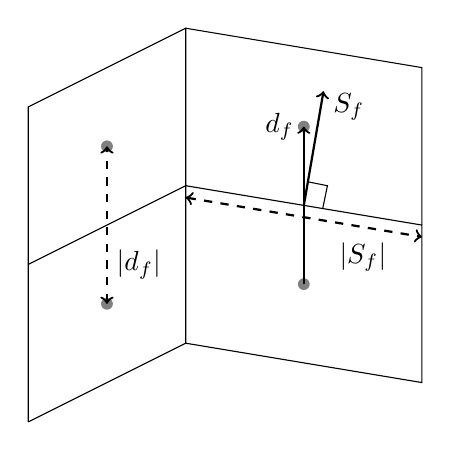
\begin{tikzpicture}[
  scale=0.5,
  cpnt/.style={fill=gray},
  arr/.style={thick, ->},
  mag/.style={dashed, thick, <->}
]
\draw (0,0) --  (4,2)  -- (4,6)  -- (0,4) -- (0,0);
\draw (4,2) --  (10,1) -- (10,5) -- (4,6);
\draw (0,4) --  (0,8)  -- (4,10)  -- (4,6);
\draw (10,5) -- (10,9) -- (4,10);
\path [cpnt] (2,3) circle [radius=0.15];
\path [cpnt] (2,7) circle [radius=0.15];
\path [cpnt] (7,3.5) circle [radius=0.15];
\path [cpnt] (7,7.5) circle [radius=0.15];
\draw [arr] (7,3.5) -- (7,7.5);
\draw [arr] (7,5.5) -- (7.5,8.4);
\node [left] at (7,7.5) {$\vect{d}_f$};
\node [right] at (7.5,8) {$\vect{S}_f$};
\draw [mag] (2,3) -- (2,7);
\node [right] at (2,4) {$|{\vect{d}_f}|$};
\draw [mag] (4,5.7) -- (10,4.7);
\node [below] at (8.5,4.8) {$|{\vect{S}_f}|$};
\draw (7.48,5.42) -- (7.6,6) -- (7.1,6.1);
\end{tikzpicture}
\end{document}
}
	\hfill
	\subcaptionbox{Placement of prognostic variables}[0.48\textwidth]{\documentclass[tikz]{standalone}
\usepackage{bm}
\newcommand{\vect}{\bm}
\newcommand{\del}{\nabla}

\newcommand{\trans}[1]{{#1^\star}}
\newcommand{\surface}{h}
\newcommand{\shellcmd}[1]{\texttt{#1}}
\newcommand{\diffusioncoeff}{\mathcal{D}}
\newcommand{\exner}{\Pi}
\newcommand{\courant}{\mathrm{Co}}

\begin{document}
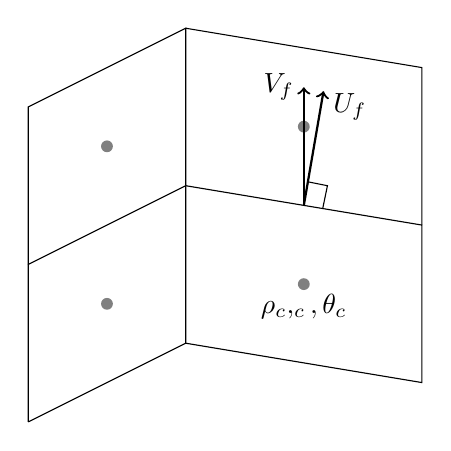
\begin{tikzpicture}[
  scale=0.5,
  cpnt/.style={fill=gray},
  arr/.style={thick, ->},
  mag/.style={dashed, thick, <->}
]
\draw (0,0) --  (4,2)  -- (4,6)  -- (0,4) -- (0,0);
\draw (4,2) --  (10,1) -- (10,5) -- (4,6);
\draw (0,4) --  (0,8)  -- (4,10)  -- (4,6);
\draw (10,5) -- (10,9) -- (4,10);
\path [cpnt] (2,3) circle [radius=0.15];
\path [cpnt] (2,7) circle [radius=0.15];
\path [cpnt] (7,3.5) circle [radius=0.15];
\path [cpnt] (7,7.5) circle [radius=0.15];
\draw [arr] (7,5.5) -- (7,8.5);
\draw [arr] (7,5.5) -- (7.5,8.4);
\node [below] at (7,3.5) {$\rho_c, \exner_c, \theta_c$};
\node [left] at (7,8.5) {$V_f$};
\node [right] at (7.5,8) {$U_f$};
\draw (7.48,5.42) -- (7.6,6) -- (7.1,6.1);
\end{tikzpicture}
\end{document}
}
	\caption{Geometric placement of prognostic variables in two dimensions.  Adapted from \textcite{weller-shahrokhi2014}.}
	\label{fig:method:placement}
\end{figure}

\TODO{pressure gradient}

\TODO{cubic upwind advection scheme}

\section{Energy measures}
\label{sec:method:energy}

Energy conservation is desirable in the discretisation of the Euler equations.  In the resting atmosphere test detailed in section~\ref{sec:resting}, energy is conserved in the analytic solution, but not in all numerical approximations.  The normalised energy change $\Delta E$ at time $t$ is found by comparing with the initial energy measure, hence
\begin{align}
	\Delta E(t) &= \frac{E(t) - E(t = \SI{0}{\second})}{E(t = \SI{0}{\second})}
\end{align}
Three energy measures are considered, where the volume integral of some field $\varphi$ is the volume-weighted sum given by
\begin{align}
	\int_V \varphi \diff{V} &= \frac{\sum_c \varphi_c V_c}{\sum_c V_c}
\end{align}
First, kinetic energy $E_K$ is calculated as \TODOcite
\begin{align}
	E_K(t) &= \int_V \frac{1}{4} \sum_{f \in \: c} \frac{\vect{u} \cdot \vect{S}_f \: \vect{u} \cdot \vect{d}_f}{V_c} \diff{V}
%
	\intertext{where \TODO{define variables if needed}  Second, potential energy $E_P$ is}
%
	E_P(t) &= - \int_V \rho \vect{g} \cdot \vect{x_c} \diff{V}
%
	\intertext{where $\vect{x}_c$ is the position vector of the centre of cell $c$.  Third, the internal energy $E_I$ is \TODOcite}
%
	E_I(t) &= \int_V \rho \theta \Pi c_v \diff{V}
\end{align}
where \TODO{define variables if needed}
